

\begin{frame}
 \frametitle{Demo 6-1 $\vert$ \bfseries Instationary heat conduction}
 \framesubtitle{\bfseries prescribed heat flux}
 \begin{overlayarea}{0.9\textwidth}{0.9\textheight}
%  \vspace*{1ex}
 \begin{center}
 \begin{tikzpicture}[scale=1.2]
  \onslide<1>{
  \fill[gray!10, draw=black] (0, 3) rectangle (3, 0) node[above left, black]{$\mathcal{B}$};
  }

  \onslide<1->{\fill[gray] (0.0, 0.0) rectangle (-0.05, 3.0);}
  \onslide<1>{\draw (-0.05, 1.5) node[above, rotate=90] {$\theta^p=25^\circ\mathrm{C}$};}
  
  \onslide<1>{
  \draw[thin,gray] (0, 0) -- +(0, -0.5);
  \draw[thin,gray] (3, 0) -- +(0, -0.5);
  \draw[<->,thin,gray] (0, -0.4) -- node[fill=white]{$\ell$} +(3, 0);
  \draw[thin,gray] (3, 0) -- +(2, 0);
  \draw[thin,gray] (3, 3) -- +(2, -0);
  \draw[<->,gray] (4.9, 0) -- node[fill=white,sloped]{$\ell$} +(0, 3);

   \draw[thick,-latex] (0,0) -- +(1, 0) node[below]{$\v e_1$};
   \draw[thick,-latex] (0,0) -- +(0, 1) node[right]{$\v e_2$};
  }
  
  \onslide<1>{
  \foreach \y in {0.0, 0.25,0.5,...,3.0}
  \draw[decorate,decoration={snake, amplitude=1pt, segment length=5pt, post length=3pt},-latex] (3.2+\y/3.0, 0.05+2.9/3.0*\y) -- +(-0.2-\y/3.0, 0);  
%   \draw (0.05, 1.5) -- node[above]{$10 \,\mathrm{MPa}$} +(2.9, 0);
%   \draw (0.05, 1.5) -- +(2.9, 0);
  \node at (3.9, 1.0) [above,yshift=0.0cm]{$q^p$};
%   \foreach \a in {0.0,45.0,90.0,...,315.0}
%   \draw[decorate,decoration={snake, amplitude=1pt, segment length=5pt, post length=3pt},-latex,xshift=0.75cm, yshift=0.75cm] (\a:0.05cm) -- (\a:0.3cm);
%   \node at (1.3, 0.5) {$r(t)$};
%   \draw[dashed,->] (1.15, 0.75) -- (2.2, 0.75);
%   \draw[dashed,->] (2.25, 0.8) -- (2.25, 2.2);
%   \draw[dashed,->] (2.2, 2.25) -- (0.8, 2.25);
%   \draw[dashed,->] (0.75, 2.2) -- (0.75, 1.15);
  }

%   \onslide<2>{
%   \node at(1.5,0.5) {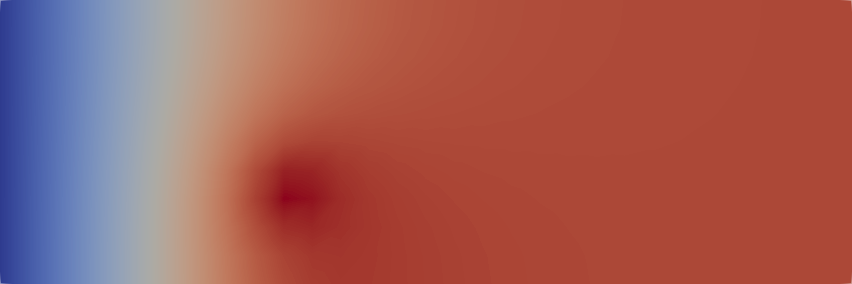
\includegraphics[width=6cm]{../02-thermo-static/01-heatsource/plot.png}};
%   \begin{scope}[xshift=3.5cm,yshift=1.3cm,scale=0.5]
%    \begin{axis}[thermobar,point meta min=0.0,point meta max=36.0,title={$\theta$ in $^\circ\mathrm{C}$}] 
%     \addplot [draw=none] coordinates {(0,0)}; \end{axis}
%   \end{scope}   
%   }

  \end{tikzpicture}
  \end{center}
  
   \onslide<1>{
   \vspace*{-5ex}
   \begin{align*}
%    \rho &= 8000 \, \tfrac{\mathrm{kg}}{\mathrm{m}^3} \\
   \kappa &= 20 \, \tfrac{\mathrm{W}}{\mathrm{m} \cdot \mathrm{K}} \\
   c_v &= 4.0 \, \tfrac{\mathrm{MW}}{\mathrm{m}^3 \cdot \mathrm{K}} \\
   \ell &= 0.1\,\mathrm{m} & q^p &= 100 \, \tfrac{x_2}{\ell} \, \tfrac{\mathrm{kW}}{\mathrm{m}^2} 
%    T &= 1 \, \mathrm{h}
   \end{align*}
   }

 \end{overlayarea}
\end{frame}

\begin{frame}{}
 \frametitle{Demo 6-1 $\vert$ \bfseries Instationary heat conduction -- Video}
 \framesubtitle{\bfseries prescribed heat flux}
  \href{../videos/lkm-demo-6-1-heatflux.avi}{
    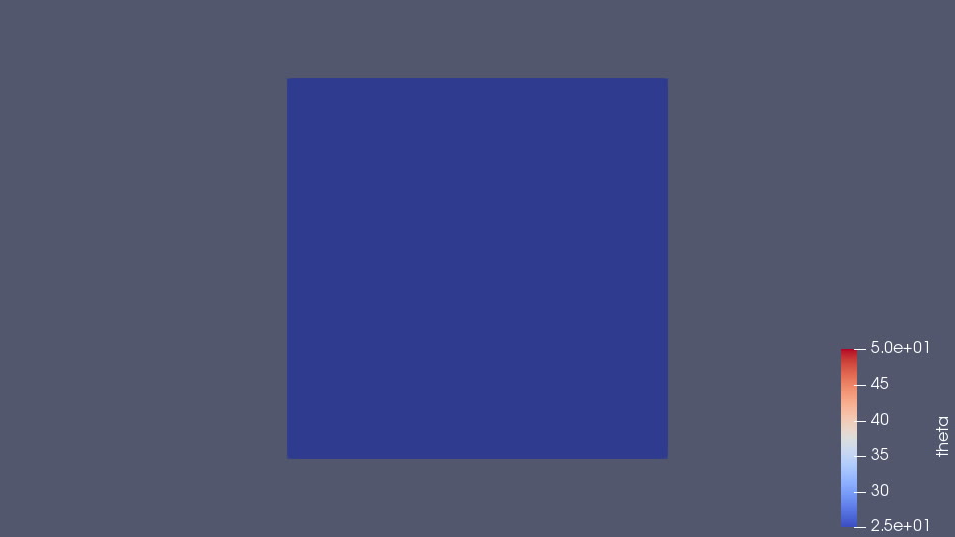
\includegraphics[scale=.3]{../videos/lkm-demo-6-1-heatflux.png}
  }
\end{frame}


\begin{frame}
 \frametitle{Demo 6-2 $\vert$ \bfseries Instationary heat conduction}
 \framesubtitle{\bfseries time-dependent heat source (selective electron beam melting)}
 \begin{overlayarea}{0.9\textwidth}{0.9\textheight}
%  \vspace*{1ex}
 \begin{center}
 \begin{tikzpicture}[scale=1.2]
  \onslide<1>{
  \fill[gray!10, draw=black] (0, 3) rectangle (3, 0) node[above left, black]{$\mathcal{B}$};
  }

%   \onslide<1->{\fill[gray] (0.0, 0.0) rectangle (-0.05, 3.0);}
%   \onslide<1>{\draw (-0.05, 1.5) node[above, rotate=90] {$\theta^p=25^\circ\mathrm{C}$};}
  
  \onslide<1>{
  \draw[thin,gray] (0, 0) -- +(0, -0.5);
  \draw[thin,gray] (3, 0) -- +(0, -0.5);
  \draw[<->,thin,gray] (0, -0.4) -- node[fill=white]{$\ell$} +(3, 0);
  \draw[thin,gray] (3, 0) -- +(0.5, 0);
  \draw[thin,gray] (3, 3) -- +(0.5, -0);
  \draw[<->,gray] (3.4, 0) -- node[fill=white,sloped]{$\ell$} +(0, 3);

   \draw[thick,-latex] (0,0) -- +(1, 0) node[below]{$\v e_1$};
   \draw[thick,-latex] (0,0) -- +(0, 1) node[right]{$\v e_2$};
  }
  
  \onslide<1>{
%   \foreach \y in {0.0, 0.25,0.5,...,1.0}
%   \draw[decorate,decoration={snake, amplitude=1pt, segment length=5pt, post length=3pt},-latex] (3.5, 0.05+0.9/1.0*\y) -- +(-0.5, 0);  
% %   \draw (0.05, 1.5) -- node[above]{$10 \,\mathrm{MPa}$} +(2.9, 0);
% %   \draw (0.05, 1.5) -- +(2.9, 0);
%   \node at (3.5, 1.0) [above,yshift=0.0cm]{$q^p$};
  \foreach \a in {0.0,45.0,90.0,...,315.0}
  \draw[decorate,decoration={snake, amplitude=1pt, segment length=5pt, post length=3pt},-latex,xshift=0.75cm, yshift=0.75cm] (\a:0.05cm) -- (\a:0.3cm);
  \node at (1.3, 0.5) {$r(t)$};
  \draw[dashed,->] (1.15, 0.75) -- (2.2, 0.75);
  \draw[dashed,->] (2.25, 0.8) -- (2.25, 2.2);
  \draw[dashed,->] (2.2, 2.25) -- (0.8, 2.25);
  \draw[dashed,->] (0.75, 2.2) -- (0.75, 1.15);
  }

%   \onslide<2>{
%   \node at(1.5,0.5) {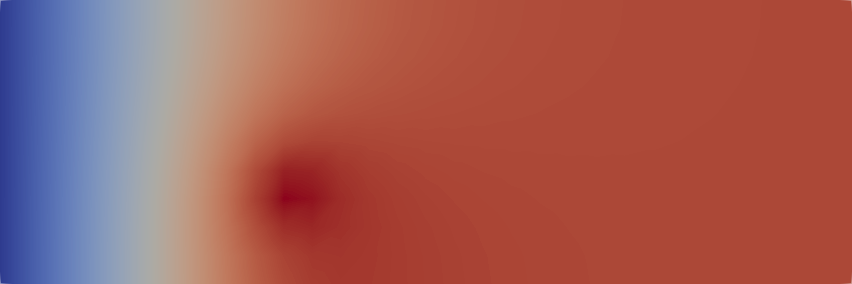
\includegraphics[width=6cm]{../02-thermo-static/01-heatsource/plot.png}};
%   \begin{scope}[xshift=3.5cm,yshift=1.3cm,scale=0.5]
%    \begin{axis}[thermobar,point meta min=0.0,point meta max=36.0,title={$\theta$ in $^\circ\mathrm{C}$}] 
%     \addplot [draw=none] coordinates {(0,0)}; \end{axis}
%   \end{scope}   
%   }

  \end{tikzpicture}
  \end{center}
  
   \onslide<1>{
   \vspace*{-5ex}
   \begin{align*}
%    \rho &= 4500 \, \tfrac{\mathrm{kg}}{\mathrm{m}^3} \\
   \kappa &= 6.6 \, \tfrac{\mathrm{W}}{\mathrm{m} \cdot \mathrm{K}} && \text{(TiAl6V4)} \\
   c_v &= 2.9 \, \tfrac{\mathrm{MW}}{\mathrm{m}^3 \cdot \mathrm{K}} \\
   \ell &= 0.5\,\mathrm{m} && r(t) = 100 \,\exp \big(-\tfrac{\vert \v x - \v x_0(t) \vert^2}{0.001 \, \ell^2} \big) \tfrac{\mathrm{MW}}{\mathrm{m}^3}
   \end{align*}
   }

 \end{overlayarea}
\end{frame}


\begin{frame}{}
 \frametitle{Demo 6-2 $\vert$ \bfseries Instationary heat conduction -- Video}
 \framesubtitle{\bfseries time-dependent heat source (selective electron beam melting)}
  \href{../videos/lkm-demo-6-2-SEBM.avi}{
    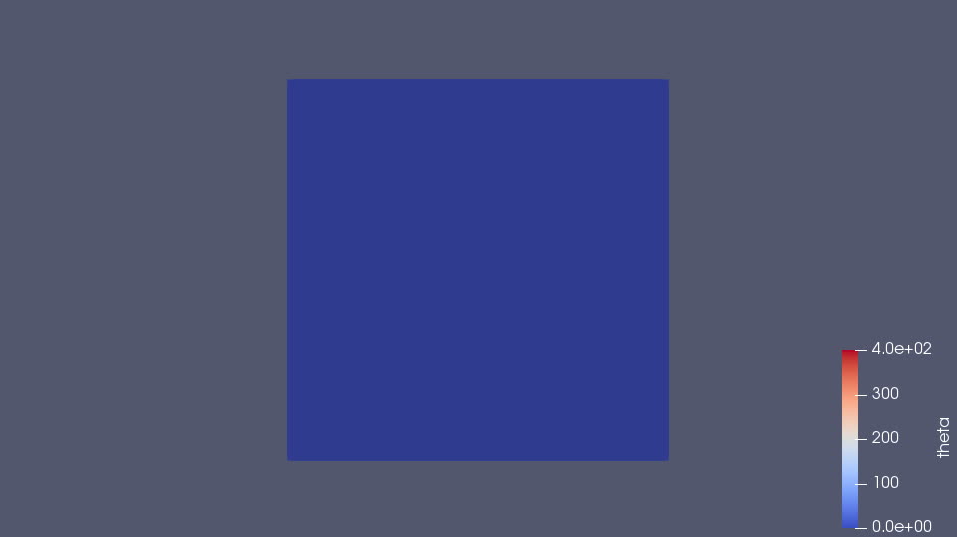
\includegraphics[scale=.3]{../videos/lkm-demo-6-2-SEBM.png}
  }
\end{frame}


\begin{frame}{}
 \frametitle{Demo 6-2 $\vert$ \bfseries Instationary heat conduction -- Video}
 \framesubtitle{\bfseries time-dependent heat source (selective electron beam melting of TiAl6V4)}
  \href{../videos/lkm-demo-6-2-extra_SLM_TiAl6V4_halfmodel.avi}{
    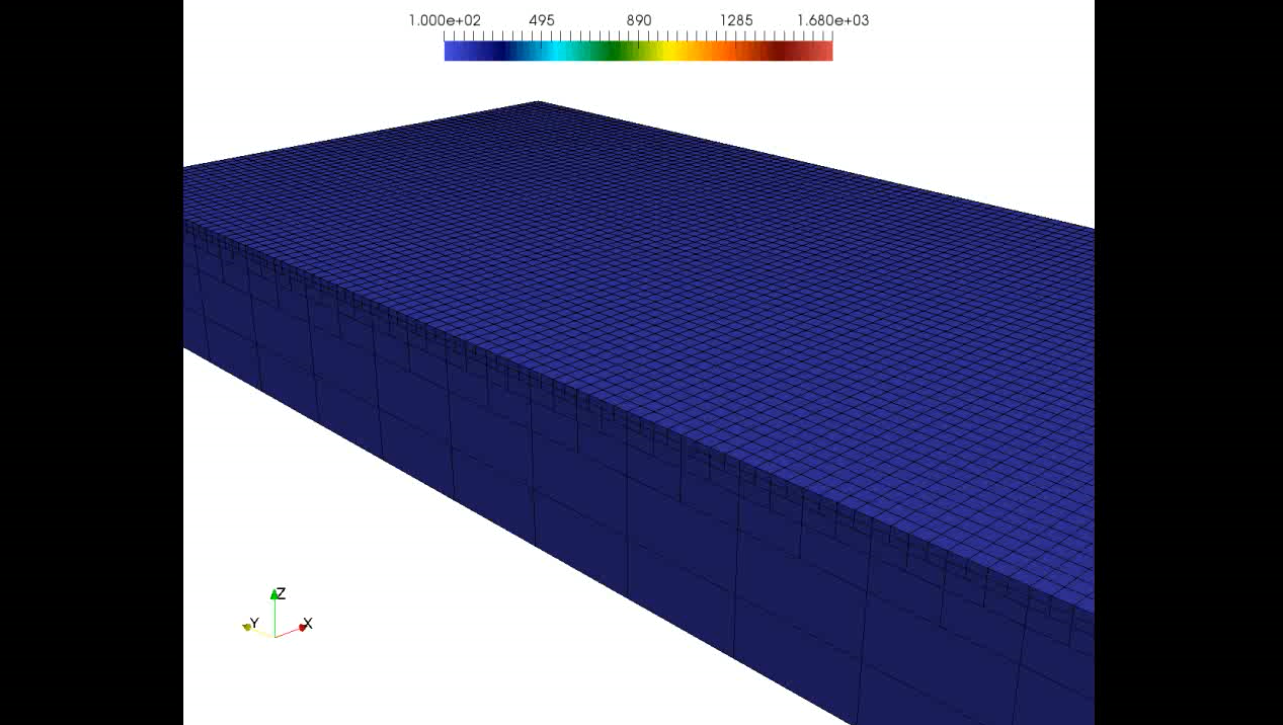
\includegraphics[scale=.23]{../videos/lkm-demo-6-2-extra_SLM_TiAl6V4_halfmodel.png}
  }
\end{frame}


